% Tesis ITAM CLASS -- version 0.1 (13 - Abr - 2015)
% Clase para las tesis del ITAM
% 
% 13 - Abr - 2015 	Victor Martinez 	victor.martinez (at) itam.mx
% LICENSE: Creative Commons SA-BY 3.0
%
%
% Este documento presenta un ejemplo de uso de la plantilla
% El estudiante es libre de modificar este archivo a su gusto
% 
\documentclass{tesisITAM}
\usepackage[utf8]{inputenc}
\usepackage{amsfonts}
\usepackage{amsmath}
%\usepackage{algorithmx}
\usepackage[spanish,onelanguage]{algorithm2e} 
\RestyleAlgo{boxruled} % Para que los algoritmos los ponga en caja

%\usepackage[group-separator={,}]{siunitx}
\usepackage{numprint}

\title{Tesis de Mario}
\author{Mario Humberto Becerra Contreras}
\degree{Licenciado en Matemáticas Aplicadas}
\advisor{Fernando Esponda Darlington}
\year{2016}

\begin{document}
	\npthousandsep{,}
	\pagenumbering{gobble}
	\maketitle
	\publicationrights

	%%%%%%%%%%%%%%%%%%%%%%%%%%%%%%%%%%%%%%%%%%%%%%
	% ABSTRACT
	%%%%%%%%%%%%%%%%%%%%%%%%%%%%%%%%%%%%%%%%%%%%%%

	\begin{abstract}{spanish}
		Este documento presenta una plantilla para usar en las tesis y tesinas del ITAM. Se provee de manera gratuita y sin ninguna responsabilidad bajo la licencia \emph{creative commons BY-SA 3.0}.
	\end{abstract}

	\selectlanguage{spanish}
	\setcounter{page}{1}
	\pagenumbering{roman}

	\tableofcontents
	\listoffigures
	\listoftables
	\newpage

	\pagenumbering{arabic}
	\setcounter{page}{1}

	%%%%%%%%%%%%%%%%%%%%%%%%%%%%%%%%%%%%%%%%%%%%%%
	% CONTENT
	%%%%%%%%%%%%%%%%%%%%%%%%%%%%%%%%%%%%%%%%%%%%%%

	\chapter{Introducción}
\label{ch:intro}

\begin{chapterquote}{Chris Anderson}
	A Long Tail is just culture  unfiltered by economic scarcity.
\end{chapterquote}

Con la cantidad de información que se genera hoy en día y la cantidad de servicios \textit{online} que tenemos, para explotar el fenómeno conocido como \textit{long tail} en \textit{marketing} los proveedores de estos servicios quieren personalizar el contenido que ofrecen a sus usuarios; en particular quieren predecir la respuesta del usuario a distintas opciones. A este tipo de sistemas se les conoce como \textbf{sistemas de recomendación}, y tal vez el más conocido es el de \textit{Netflix}; sin embargo, existen más, como la sección de 'Qué ver' en \textit{YouTube} o los destinos que nos recomiendan en \textit{Airbnb} o lo productos que nos recomiendan en \textit{Amazon}.

Los sistemas de recomendación se han vuelto más populares últimamente por varias razones, pero todo se podría resumir en un solo concepto: \textit{long tail} o cola larga. Este concepto rompe la creencia del principio de Pareto que afirma que el 80\% de las consecuencias (ganancias) provienen del 20\% de las causas (productos). Este principio se ha usado como regla de dedo en distintas disciplinas, pero en ciertos productos no se cumple, por ejemplo, las rentas de películas en \textit{Netflix}, las cuales tienen una cola larga. En una distribución de cola larga, es menos del 80\% de las ganancias el que proviene del 20\% de los productos, esto significa que se pueden tener ganancias a partir de productos no tan populares. Se puede ver una imagen de una distribución de cola larga en la figura~\ref{fig:longtailimg}.

Con el concepto de cola larga en mente, podemos imagina por qué un sistema de recomendación puede servir para ciertos tipos de productos como \textit{Netflix} o \textit{Amazon}. Estas empresas tienen miles y miles de distintos productos que ofrecer, y muchos de ellos no son populares o conocidos por la mayoría de los usuarios, entonces, mediante un sistema de recomendación, se les pueden ofrecer productos no conocidos por ellos pero que pueden ser de su agrado. Esto le funcionó bastante bien a \textit{Netflix}, pues en un principio, el 30\% de sus rentas provenía de estrenos, comparado con el 70\% de \textit{Blockbuster}; y esto era en parte gracias al sistema de recomendación, y a que \textit{Netflix}, a diferencia de \textit{Blockbuster}, no tenía el espacio limitado para guardar películas físicamente.

Un ejemplo extremo de la aplicación de los sistemas de recomendación y de la cola larga es el libro \textit{Touching the Void}. Este libro no fue muy popular cuando acababa de salir, pero años después un libro parecido llamado \textit{Into Thin Air} fue publicado. Ambos eran vendidos por \textit{Amazon}, y su sistema de recomendación encontró algunas personas que compraron ambos libros y empezó a recomendar \textit{Touching the Void} a usuarios que habían comprado o considerado comprar \textit{Into Thin Air}, y eventualmente \textit{Touching the Void} se volvió popular.

\begin{figure}
  \centering
    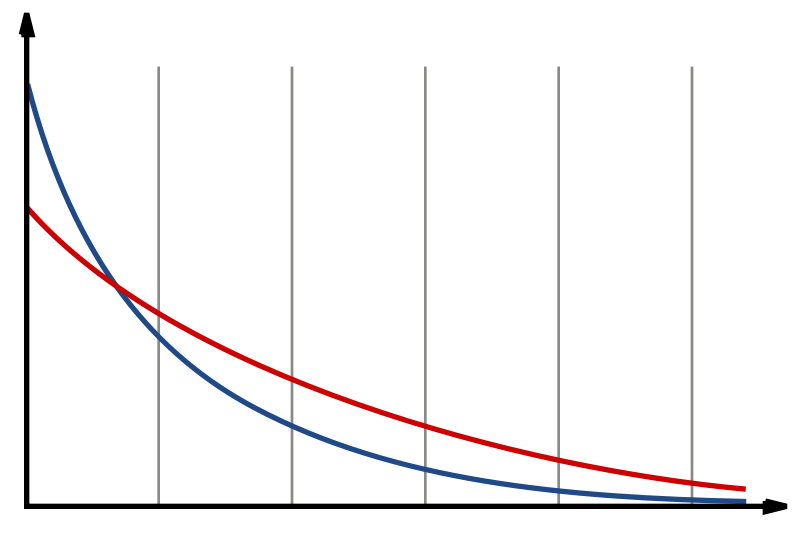
\includegraphics[width=0.5\textwidth]{LongTail.png}
  \caption{Una distribución de cola larga (roja) con una de cola no larga (azul).}
  \label{fig:longtailimg}
\end{figure}
	
	%!TEX root = ../tesis_mbc.tex

\chapter{Marco teórico}

\section{Aprendizaje estadístico}

El aprendizaje estadístico se refiere a un conjunto de herramientas para modelar y entender conjuntos de datos complejos. Es un área relativamente moderna, y tiene componentes de computación, en particular del aprendizaje de máquina. Aunque estas disciplinas van de la mano, no son totalmente equivalentes, teniendo ciertas diferencias filosóficas en cuanto a qué se hace en cada una.

Con la enorme cantidad de datos a los que se tiene acceso ahora, el aprendizaje estadístico se ha vuelto un campo muy demandado y fructífero en muchas áreas. El progreso que se ha logrado en los últimos años se ha debido en gran parte al desarrollo del poder de cómputo, sin el cual muchas de las técnicas modernas sería imposible tener un resultado.

Usualmente se divide al aprendizaje estadístico en dos vertientes: aprendizaje supervisado y aprendizaje no supervisado. El primero involucra construir un modelo estadístico para predecir o estimar una variable llamada \textit{de respuesta} basado en una o más variables llamadas \textit{de entrada}; mientras que en el aprendizaje no supervisado se tienen variables de entrada pero no de salida, se desea aprender relaciones y estructura de los datos.

Un ejemplo de aprendizaje supervisado es estimar el ingreso de un hogar a partir de variables acerca de la zona en donde se habita, tipo de casa en la que se vive, número de carros, etc. Y un ejemplo de aprendizaje no supervisado sería encontrar grupos de los hogares que surjan naturalmente a partir de los datos, de tal forma que dentro de cada grupo exista una gran similitud (definida \textit{a priori}) y entre los grupos haya diferencias. Gran parte del problema aquí radica en definir la medida de similitud.

\subsection{Aprendizaje supervisado}

Como se mencionó, en el aprendizaje supervisado, se tiene una variable respuesta, la cual será denotada como el vector $Y$ de dimensión $n$, y cada variable de entrada se denomina $X_i$, con $i$ desde $0$ hasta $p$. Cada $X_i$, al igual que $Y$, es un vector de dimensión $n$, por lo que el conjunto de datos $\left \{ X_1, ..., X_p \right \}$ se puede escribir como una matriz  $X = \left[ X_1, ..., X_p \right ]$ de dimensiones $n \times p$. Se asume que existe una relación entre $Y$ y $X$ que se puede escribir de forma general como
$$Y = f(X) + \varepsilon.$$

Aquí, $f$ es una función de $X$ fija pero desconocida, la cual tiene información sistemático de $X$ acerca de $Y$, y $\varepsilon$ es un término de error aleatorio. La esencia del aprendizaje supervisado es poder encontrar o aprender $f$ a partir del \textit{conjunto de entrenamiento} denominado $\mathcal{L}$, tal que $\mathcal{L} = \left\{ (x_1, y_1), ..., (x_n, y_n) \right\}$. En este caso, cada $y_i$ es un escalar y cada $x_i$ es un vector de dimensión $p$. Con $\mathcal{L}$ se construye un predictor $\hat{f}$, que es una estimación de $f$, de tal forma que se tiene una estimación $\hat{Y}$ de $Y$ aplicando $X$ a $\hat{f}$, es decir

$$\hat{Y} = \hat{f}(X).$$

La estimación $\hat{f}$ se hace seleccionando $f$ de una familia de funciones $\mathcal{F}$ de tal forma que $y_i \approx \hat{f}(x_i)$ para cada $(x_i, y_i) \in \mathcal{L}$. Por ejemplo, en regresión lineal se resuelve el problema de mínimos cuadrados

$$\hat{f} = \argmin_{f \in \mathcal{F}} \frac{1}{n} \sum_{i = 1}^n{ ( y_i - f(x_i) ) ^ 2},$$

donde $\mathcal{F}$ es la familia de funciones de la forma $f(X) = X\beta$ con $\beta \in \mathbb{R}^p$. Así, $\hat{f}(X) = X \hat{\beta}$, donde $\hat{\beta}$ resuelve el problema de mínimos cuadrados. En este caso, se quiere encontrar el vector de parámetros $\beta$ tal que la suma de residuales al cuadrado sea mínima.

Si la familia de funciones $\mathcal{F}$ es muy inflexible (como regresión lineal), entonces las predicciones tenderán a ser malas pues no se capta bien la relación entre $X$ y $Y$, sin embargo, esto puede ser deseable en algunos casos, como cuando se pretende interpretar la relación entre $X$ y $Y$.

Es prudente introducir el concepto de \textit{función de pérdida} o de error. Sea $\hat{Y} = \hat{f}(X)$, la predicción de $Y$; en el caso de regresión lineal, $\hat{Y} = X\hat{\beta}$. En este mismo caso la función de pérdida fue la de pérdida cuadrática, definida como 
%$L_{\mathcal{L}}(f, \hat{f}) = (f - \hat{f}_{\mathcal{L}} ) ^2$
$L_{\mathcal{L}}(\hat{Y}, Y) = (\hat{f}(X) - Y ) ^2$
, o sea, la diferencia entre la estimación de $Y$ y la verdadera $Y$ al cuadrado, con los datos del conjunto $\mathcal{L}$. Existen distintos tipos de funciones de pérdida, pero muchas veces se utiliza la pérdida cuadrática debido a las propiedades diferenciables que tiene.

En general, cuando uno entrena un modelo para predecir, no se desea minimizar el error de entrenamiento $L_{\mathcal{L}}$, sino el error de predicción, esto es, el error de cualquier observación futura $(X^0, Y^0)$. Esto quiere decir que no se quiere minimizar $L_{\mathcal{L}}(f, \hat{f})$, sino el error esperado de predicción, definido como $\mathbb{E} \left[ L(\hat{f}(X^0), Y^0 ) \right] $.

Debido a que se quiere minimizar el error esperado de predicción, es común separar el conjunto de datos $(X, Y)$ en dos, el conjunto de entrenamiento, presentado anteriormente como $\mathcal{L}$, y un \textit{conjunto de validación} o \textit{conjunto de prueba} denotado como $\mathcal{T}$. Para hacer esto, del conjunto original de datos, se toma una muestra aleatoria para entrenar (este es el conjunto de entrenamiento $\mathcal{L}$) y el resto es el conjunto de validación $\mathcal{T}$, con el cual se prueba el poder predictivo del modelo. A $L_{\mathcal{T}}$ se le conoce como el error de validación o error de prueba, y es una estimación del error de predicción. Si $\mathcal{T}$ tiene $m$ elementos, y $m$ es grande, entonces el error de prueba se aproxima al error esperado de predicción.

Notar que el error de entrenamiento no aproxima el error de predicción porque el error de entrenamiento depende de $\mathcal{L}$. De hecho la predicción del error de predicción utilizando el error de entrenamiento está sesgada hacia abajo, especialmente para modelos complejos.

\subsubsection{Regresión y clasificación}

El aprendizaje supervisado, a su vez, puede ser dividido en dos tipos de problemas dependiendo del tipo de variable respuesta. Cuando la variable respuesta es categórica, se dice que es un problema de clasificación, en otro caso, se dice que es un problema de regresión. Un ejemplo de problema de regresión es modelar el precio de una casa, mientras que un ejemplo de problema de clasificación es modelar el género de una persona. 

\subsection{Aprendizaje no supervisado}

El aprendizaje no supervisado describe un problema más retador en cuanto a que para cada $i = 1, .., n$, se tiene un vector de observaciones $x_i$ para el cual no se tiene una respuesta asociada $y_i$. Es por esto que se le llama \textit{no supervisado}, pues no hay una variable respuesta en el análisis. Uno de los principales análisis que se hace en el aprendizaje no supervisado es \textit{análisis de conglomerados}, en el cual a cada una de las observaciones $x_1, ..., x_n$ se clasifica en un grupo. Existen muchos métodos de análisis de conglomerados, sin embargo, no es el objetivo de este trabajo estudiarlas.


\subsection{Regularización}

\subsection{Evaluación de desempeño}

\section{Optimización de funciones de pérdida}

\subsection{Descenso en gradiente}

\subsection{Descenso en gradiente estocástico}

\section{Sistemas de recomendación}

El objetivo de los sistemas de recomendación es predecir las respuestas de los usuarios a distintas opciones. Dos clasificaciones muy amplias de los sistemas de recomendación son: basados en contenido y filtrado colaborativo. Existen dos grandes tipos de sistemas de recomendación de acuerdo a las técnicas que usan.

\begin{itemize}
\item Basados en contenido: A partir de características y propiedades de los productos (por ejemplo, género, actores, país de origen, año, etc.) intentamos predecir el gusto por el producto construyendo variables derivadas del contenido de los artículos (como qué actores salen, año, etc.).
\item Colaborativos: A partir de usuarios y productos se construyen medidas de similitud en el sentido de que les han gustado los mismos productos o que les gustaron a las mismas personas. Así, los productos recomendados a un usuario son los que le gustaron a otros usuarios.
\end{itemize}

En este trabajo se supone que se tiene una matriz de calificaciones $R$, tal que las filas representan usuarios que calificaron a los productos representados en las columnas de la siguiente forma:

\begin{center}
\begin{tabular}{ c | c  c c c c}
    & $P_1$ & $P_2$ & $P_3$ & $\cdots$ & $P_n$ \\
  \hline                       
  $U_1$ &   1 &     2 &     3 & $\cdots$ &      - \\
  $U_2$ &   4 &     - &     4 & $\cdots$  &     -\\
  $\vdots$ & $\vdots$ & $\vdots$ & $\vdots$ & $\ddots$ & $\vdots$\\
  $U_m$ &   - &     - &     1 & $\cdots$ &      3\\
  \hline  
\end{tabular}
\end{center}

donde cada $P_i$ es el producto i-ésimo que se ofrece y $U_i$ es el usuario i-ésimo que ha calificado el producto correspondiente. Los espacios donde hay guiones representan datos faltantes. Es usual que este tipo de matrices tengan la mayor parte de las entradas faltantes, pues no todos los usuarios han visto todas las películas, o calificado todos los productos. El objetivo del sistema de recomendación es llenar los espacios faltantes mediante una predicción y recomendar los productos que tienen una predicción alta. Notar que aquí se considera que ya se tiene la matriz de calificaciones, lo cual a veces, en la práctica, puede ser un trabajo difícil y haya que pedir a usuarios que califiquen productos.

\subsection{Basados en contenido}

Para este tipo de recomendaciones se construye un \textbf{perfil} para cada producto. Como se había mencionado, este perfil puede contener el género, los actores, país de origen, etc. Esto puede ser más sencillo en el caso de películas pues existen fuentes de información sobre las películas como \textit{Internet Movie Database (IMDb)}; pero con documentos o imágenes, por ejemplo, no siempre se tiene esta información, así que es necesario la construcción de variables a través de \textit{tags}, palabras clave y, en el caso de texto, tal vez un modelo de lenguaje.

Una vez construidos los perfiles, el proceso que queda es de alguna forma emparejar los gustos del usuario obtenidos de la matriz de utilidad con los perfiles de los productos.

Un ejemplo muy sencillo es el siguiente. Imaginemos dos películas con 5 actores cada una y que dos actores están en las dos películas, y que además las calificaciones promedio de cada película son 3 y 4. Entonces los perfiles de dos películas se ven como:

\begin{center}
\begin{tabular}{ c | c  c c c c c c c c}
    & Actor 1 & Actor 2 & Actor 3 & Actor 4 & Actor 5 & Actor 6 & Actor 7 & Actor 8 & Calif \\ \\
  \hline                       
$P_1$ & 0 & 1 & 1 & 0 & 1 & 1 & 0 & 1 & 3 \\
$P_2$ & 1 & 1 & 0 & 1 & 0 & 1 & 1 & 0 & 4 \\
  \hline  
\end{tabular}
\end{center}

Con esta información se puede obtener una medida de similitud entre las películas. Una medida muy utilizada es la distancia coseno, definida como

\begin{equation}
sim(P_1, P_2) = \dfrac{P_1 \cdot P_2}{\vert \vert P_1 \vert \vert \times \vert \vert P_2 \vert \vert}
\end{equation}

Dos películas son más similares si tienen una distancia coseno menor.

Supongamos ahora que los usuarios $U_k$ y $U_j$ solo han calificado dos película. Si el usuario $U_k$ calificó con 2 y 4 las películas $P_1$ y $P_2$ respectivamente y si el usuario $U_j$ calificó con 4 y 4 las películas $P_1$ y $P_2$ respectivamente, entonces se puede ver esto en forma matricial.

\begin{center}
\begin{tabular}{ c | c  c }
    & $P_1$ & $P_2$ \\ \\
  \hline                       
$U_k$ & 2 & 4 \\
$U_j$ & 4 & 4 \\
  \hline  
\end{tabular}
\end{center}

Tiene sentido centrar las calificaciones por usuario (restarle la media) para reducir un poco la heterogeneidad de la escala, entonces tenemos

\begin{center}
\begin{tabular}{ c | c  c }
    & $P_1$ & $P_2$ \\ \\
  \hline                       
$U_k$ & -1 & 1 \\
$U_j$ & 0 & 0 \\
  \hline  
\end{tabular}
\end{center}

Así, para el usuario $U_k$ tenemos que los perfiles para cada película se ven como

\begin{center}
\begin{tabular}{ c | c  c c c c c c c c}
    & Actor 1 & Actor 2 & Actor 3 & Actor 4 & Actor 5 & Actor 6 & Actor 7 & Actor 8 & Calif \\ \\
  \hline                       
$P_1$ & 0 & -1 & -1 & 0 & -1 & -1 & 0 & -1 & 2 \\
$P_2$ & 1 & 1 & 0 & 1 & 0 & 1 & 1 & 0 & 4 \\
  \hline  
\end{tabular}
\end{center}

Y para el usuario $U_j$ tenemos que los perfiles para cada película se ven como

\begin{center}
\begin{tabular}{ c | c  c c c c c c c c}
    & Actor 1 & Actor 2 & Actor 3 & Actor 4 & Actor 5 & Actor 6 & Actor 7 & Actor 8 & Calif \\ \\
  \hline                       
$P_1$ & 0 & 4 & 4 & 0 & 4 & 4 & 0 & 4 & 4 \\
$P_2$ & 4 & 4 & 0 & 4 & 0 & 4 & 4 & 0 & 4 \\
  \hline  
\end{tabular}
\end{center}

Entonces, para el perfil general de cada usuario, se promedian por película los perfiles de cada uno y obtenemos

\begin{center}
\begin{tabular}{ c | c  c c c c c c c c}
    & Actor 1 & Actor 2 & Actor 3 & Actor 4 & Actor 5 & Actor 6 & Actor 7 & Actor 8 & Calif \\ \\
  \hline                       
$U_k$ & 0.5 & 0 & -0.5 & 0.5 & -0.5 & 0 & 0.5 & -0.5 & 3 \\
$U_j$ & 2 & 4 & 2 & 2 & 2 & 4 & 2 & 2 & 4 \\
  \hline  
\end{tabular}
\end{center}

Con esto podemos estimar qué tanto le va a gustar a un usuario una película calculando la distancia coseno entre el perfil del usuario y el perfil de la película. Esta forma es muy rudimentaria y sencilla, pero puede servir como base para otros modelos.

\subsection{Colaborativos}

\subsubsection{Modelo base} \label{sec:modelo_base}

En esta sección se construye un modelo base muy sencillo para hacer predicciones, y el cual sirve como comparación con otros modelos más complejos. Para este modelo se supone que los artículos y los usuarios tienen sesgos, o sea, hay usuarios que tienden a calificar más alto, o a ser más estrictos y calificar más bajo; al mismo tiempo, puede haber artículos que tiendan a recibir calificaciones más altas; y que gran parte de la calificación observada se debe a efectos asociados a estos sesgos.

Sea $\mu$ la media general de todos los artículos y todos los usuarios, entonces la predicción del modelo base es

\[
\hat{r_{ij}} = \mu + a_i + b_j
\]

donde $a_i$ es la desviación del usuario $i$ respecto a la media general y $b_j$ es la desviación del artículo $j$ respecto a la media general.

Una forma de estimar los sesgos es calculando

\[
a_i = \frac{1}{M_i} \sum_t r_{it} - \mu,
\]
y 
\[
b_j = \frac{1}{N_j} \sum_s r_{sj} - \mu,
\]
donde donde $M_i$ es el número de artículos calificados por el usuario $i$ y $N_j$ es el número de calificaciones que tiene el artículo $j$.

Otra forma un poco más precisa es resolver el problema de mínimos cuadrados

\[
\min_{b} \sum_{(i, j) \in A} \left( r_{ij} - \mu - a_i - b_j \right) ^2 + \lambda \left( \sum_{i} a_i^2 + \sum_{j} b_j^2 \right)
\]

donde $r_{ij}$ es la calificación del usuario $i$ del artículo $j$, $A$ es el conjunto de usuarios y artículos para los cuales se conoce la calificación $r_ij$, $ \vert A \vert$ es la cardinalidad de $A$ (o sea, el total de artículos calificados por todos los usuarios) y $\lambda$ es un término de regularización que evita el sobreajuste.

A este sencillo modelo se le pueden agregar otros términos de regularización que ayuden a disminuir el ruido causado por artículos y usuarios con pocas calificaciones, al encoger las calificaciones a la media. Una vez que se calcularon $a_i$ y $b_j$ usando cualquiera de los métodos mencionados, se hace la predicción

\[
r_{ij} = \mu + \frac{M_i}{\gamma + M_i} a_i + \frac{N_j}{\gamma + N_j}b_j
\]

donde $M_i$ es el número de artículos que ha calificado el usuario $i$, $N_j$ es el número de calificaciones que tiene el artículo $j$, y $\gamma$ es el parámetro de regularización.

\subsubsection{Métodos de vecindario}

Este tipo de modelos se centran en la similitud de los usuarios y los artículos. Los usuarios son similares si los vectores que los representan (es decir, las filas en la matriz de calificaciones) están cercanos de acuerdo a alguna similitud definida. Una recomendación para un usuario $i$ se hace al ver a los usuarios más parecidos a $i$ y recomendando artículos que hayan sido del agrado de estos usuarios parecidos.

El primer problema con estos métodos surge al definir una medida de similitud entre artículos o usuarios. Dos medidas muy utilizadas son la similitud de Jaccard y la similitud coseno. En el caso de una matriz de calificaciones binaria, la similitud Jaccard tendría más sentido, pero si son calificaciones explícitas conviene más utilizar similitud coseno. Una desventaja de utilizar la similitud coseno es que los elementos faltantes son tratados como $0$, lo cual tiene el efecto de tratar la falta de calificación como disgusto hacia el artículo. Una forma de solucionar esto es centrando las calificaciones por usuario al restar la media, de esta forma el faltante al ser tratado como cero tiene el efecto de que al usuario ni le gusta ni le disgusta el artículo.

Una forma de hacer predicciones de calificaciones para un usuario $i$ y un artículo $j$ es encontrar los un vecindario de los $n$ usuarios más parecidos a $i$ y tomar el promedio de las calificaciones del artículo $j$. O de forma dual, se podría encontrar un vecindario con los $n$ artículos más parecidos a $j$ y tomar el promedio de las calificaciones que el usuario $i$ ha dado a esos artículos. Aquí se hace una vertiente en los métodos de vecindario, dependiendo de si se centran en las similitudes de los usuarios o de los artículos.

\paragraph{Basados en usuarios}

Este tipo de algoritmos pretenden imitar las recomendaciones de boca en boca al asumir que los usuarios con preferencias similares calificarán los artículos de forma similar. De esta manera, para hacer una predicción para el usuario $i$ y el artículo $j$ habría que encontrar un vecindario de $i$, denotado como $N(i)$, y tomar el promedio de las calificaciones en el vecindario:

\begin{equation}\label{predic_modelo_usuario_sencillo}
 \hat{r_{ij}} = \frac{\sum_{a \in N(i)} r_{aj}}{\vert N(i) \vert}.
\end{equation}

Por ejemplo,

\textbf{PONER EJEMPLO DE CUADERNO!!!}.

Este ejemplo está ignorando el hecho de que algunos usuarios en el vecindario son más similares a otros, por lo que es una buena idea tener un ponderador de similitud. Así, en lugar de \ref{predic_modelo_usuario_sencillo}, la predicción es

\begin{equation}\label{predic_modelo_usuario_ponderado}
 \hat{r_{ij}} = \frac{\sum_{a \in N(i)} s_{ia} r_{aj}}{\sum_{a \in N(i)} s_{ia}},
\end{equation}

donde $s_{ia}$ es la similitud entre el usuario $i$ y el usuario $a$ perteneciente al vecindario de $i$.

\paragraph{Basados en artículos}

Este tipo de algoritmos asumen que los usuarios prefieren artículos que son similares a otros artículos que les gustaron. Muchas veces este tipo de sistemas producen información más confiable porque es más sencillo encontrar artículos del mismo género que encontrar usuarios a los que solo les gustan artículos de un solo género. En este caso, para hacer una predicción para el usuario $i$ y el artículo $j$ habría que encontrar un vecindario de $j$, denotado como $N(j)$, y tomar el promedio (ponderado por nivel de similitud para mejor estimación) de las calificaciones que el usuario ha hecho a los artículos en $N(j)$, es decir

\begin{equation}\label{predic_modelo_articulo_ponderado}
 \hat{r_{ij}} = \frac{\sum_{a \in N(j)} s_{ja} r_{ia}}{\sum_{a \in N(j)} s_{ja}},
\end{equation}

donde $s_{ja}$ es la similitud entre el artículo $j$ y el artículo $a$ perteneciente al vecindario de $j$.

Por ejemplo,

\textbf{PONER EJEMPLO DE CUADERNO!!!}.

\subsubsection{Métodos de factorización de matrices} \label{sec:modelo_factorizacion}

\paragraph{Modelo básico de factorización de matrices}

La idea de la factorización de matrices proviene de los modelos de factores latentes, en los cuales se supone que hay factores ocultos o latentes que caracterizan a los usuarios y a los productos. Por ejemplo, se podría suponer que las películas se pueden resumir en dos factores: una dimensión de seriedad-comedia y una dimensión de fantasía-realidad, ambas numéricas, de tal forma que en la primera dimensión un valor más alto significa que una película es más seria y más bajo significa que es más inclinada a comedia. Para la segunda dimensión, similarmente, un valor más alto significa que la película está más inclinada a fantasía y un menor valor significa que está más apegada a la realidad. Estos factores latentes también se pueden pensar para los usuarios, en el sentido de que un usuario tiene un valor más alto en la primera dimensión si le gustan más las películas serias y un valor más alto en la segunda dimensión si le gustan las películas de fantasía.

Teniendo esto en cuenta, los usuarios y las películas se pueden representar en vectores. El vector correspondiente a un usuario que le gustan mucho las películas serias de fantasía se podría ver así:

\[
     u_1 = 
    \begin{bmatrix}
        3 & 4
    \end{bmatrix}^{T}.
\]
  
Y un usuario que le gustan las comedias pero es indiferente entre si es de fantasía o realidad se podría ver así:

\[
     u_2 = 
     \begin{bmatrix}
         -2 & 0
    \end{bmatrix}^{T}.
\]
  
De la misma forma se podría pensar en dos películas, una seria con fantasía, como \textit{El Señor de los Anillos}, y una apegada a la realidad de comedia, como \textit{Mean Girls}. Sus vectores correspondientes se podrían ver así:

\[
    p_1 = 
    \begin{bmatrix}
         2 & 4
    \end{bmatrix}^{T}
\]


\[
    p_2 = 
    \begin{bmatrix}
         -3 & -3
    \end{bmatrix}^{T}.
\]

Entonces una forma de modelar la calificación que daría cada usuario a cada película sería pensando en la combinación lineal de los usuarios y las películas. Es decir, la calificación que daría el usuario $u_1$ a la película $p_1$ sería el producto punto de los vectores: $u_1^T p_1 = 22$. Si se hace esto para todos los usuarios y películas, se tiene el siguiente sistema lineal:

\[
    R = UP^T,
\]


donde

\[
    U = 
    \begin{bmatrix}
         u_1^T \\ 
         u_2^T
    \end{bmatrix} =
    \begin{bmatrix}
         3 & 4 \\ 
         -2 & 0
    \end{bmatrix},\;\;\;\;
    P = 
    \begin{bmatrix}
         p_1^T \\ 
         p_2^T
    \end{bmatrix} =
    \begin{bmatrix}
         2 & 4 \\ 
         -3 & -3
    \end{bmatrix}
\]

y

\[
    R = 
    \begin{bmatrix}
         u_1 ^T p_1 & u_1 ^T p_2 \\ 
         u_2 ^T p_1 & u_2 ^T p_2
    \end{bmatrix}
    =
    \begin{bmatrix}
        22 & -21 \\
        -4 & 6.
    \end{bmatrix}
\]

Aquí se puede ver que el usuario $u_1$, a quien le gustan las películas serias de fantasía califica más alto \textit{El Señor de los Anillos} que \textit{Mean Girls}, mientras que el usuario $u_2$ hace lo contrario, pues le gustan las comedias.

Ahora, en la vida real no se conocen los valores de las matrices $U$ y $P$, sino que se tiene acceso a ciertas entradas de la matriz $R$, y el reto está en tener una buena estimación de las matrices $U$ y $P$. Este problema es una instancia de la descomposición en valores singulares, con la peculiaridad de que no se tienen todas las entradas de la matriz R, sino solo una pequeña proporción de ellas.

Entonces, si se tiene acceso a la matriz $R$, se busca encontrar dos matrices $U$ y $P$ de rango $k$ tales que $R \approx U P^T$. De esta forma, la aproximación de la calificación que da el usuario $i$ al artículo $j$ sería

\begin{equation}\label{ec_fact_basico}
r_{ij} = u_i^T p_j.
\end{equation}


Hay distintas formas de elegir qué función de pérdida utilizar para saber qué tan cerca el producto de matrices está de $R$, pero muchas veces se utiliza la raíz del error cuadrático medio (RMSE por \textit{root-mean-squared-error}), el cual se calcula de la siguiente forma:

\[
RMSE = \left ( \frac{1}{\vert A \vert} \sum_{(i,j) \in A} (r_{ij} - u_i^Tp_j )^2 \right ) ^ \frac{1}{2},
\]

donde $r_{ij}$ es la calificación del usuario $i$ del artículo $j$, $A$ es el conjunto de usuarios y artículos para los cuales se conoce la calificación $r_ij$, $ \vert A \vert$ es la cardinalidad de $A$ (o sea, el total de artículos calificados por todos los usuarios), $u_i$ es la i-ésima fila de la matriz $U$ y $p_j$ es la j-ésima fila de la matriz $P$. Es decir, el RMSE es la raíz cuadrada del promedio de las desviaciones de la aproximación de $R$ y la $R$ verdadera. 

Otra opción muy utilizada es el error absoluto medio (MAE por \textit{mean-absolute-error}), definido como la suma de las desviaciones absolutas de la aproximación de $R$ a $R$, esto es

\[
MAE = \frac{1}{\vert A \vert} \sum_{(i,j) \in A} \vert r_{ij} - u_i^Tp_j \vert.
\]

El RMSE puede ser preferible en situaciones en las que pequeños errores de predicción no son importantes, pues el RMSE penaliza errores más fuertemente que el MAE.

Por lo tanto, cuando se quiere minimizar el RMSE, el problema a resolver es

\begin{equation}
\min_{p, u} \sum_{(i,j) \in A} \left [ (r_{ij} - u_i^Tp_j )^2 + \lambda ( \norm{p_j}^2 + \norm{u_i}^2 ) \right ]
\end{equation}

donde $\lambda$ es un término de regularización que evita el sobreajuste.

\paragraph{Agregando sesgos}

Al modelo simple enunciado en la sección anterior se le puede agregar la idea del modelo base: que existen sesgos en los artículos y en los usuarios. Entonces al modelo \ref{ec_fact_basico} se le agregan los sesgos, de tal forma que se tiene el nuevo modelo con sesgos

\begin{equation}\label{ec_fact_sesgo}
r_{ij} = \mu + a_i + b_j + u_i^T p_j,
\end{equation}

con $\mu$, $a_i$ y $b_j$ definidos anteriormente. Estos parámetros se pueden estimar resolviendo el problema

\begin{equation}\label{func_opt_sesgos}
  \min_{p, u, b, a} \sum_{(i,j) \in A} \left [ \left( r_{ij} - \mu - a_i - b_j - u_i^T p_j \right) ^2 + \lambda \left( \norm{p_j}^2 + \norm{u_i}^2 + a_i^2 + b_j^2 \right) \right ]
\end{equation}

\paragraph{Modelo de optimización}

Sea $L$ la función a optimizar en el problema \ref{func_opt_sesgos}, es decir,

\[
\begin{split}
L 
& = \sum_{(i,j) \in A} \left [ \left( r_{ij} - \mu - a_i - b_j - u_i^T p_j \right) ^2 + 
\lambda \left( \norm{p_j}^2 + \norm{u_i}^2 + a_i^2 + b_j^2 \right) \right ] \\
& = \sum_{(i,j) \in A} \left [ \left( x_{ij} - a_i - b_j - u_i^T p_j \right) ^2 + \lambda \left( \norm{p_j}^2 + \norm{u_i}^2 + a_i^2 + b_j^2 \right) \right ] \\
& = \sum_{(i,j) \in A} \left( x_{ij} - a_i - b_j - u_i^T p_j \right) ^2 \\
& + \lambda \left( 
\sum_j \sum_{m = 1}^{k}p_{jm}^2 + 
\sum_i \sum_{m = 1}^{k}u_{im}^2 + 
\sum_i a_i^2 + 
\sum_j b_j^2 \right) .
\end{split}
\]

Para utilizar descenso en gradiente estocástico, se define la función de pérdida $l_{ij}$ como

\[
l_{ij} = \left( x_{ij} - a_i - b_j - u_i^T p_j \right) ^2
+ \lambda \left( 
\sum_{m = 1}^{k}p_{jm}^2 + 
\sum_{m = 1}^{k}u_{im}^2 + 
a_i^2 + 
b_j^2 \right) .
\]

Notar que $L = \sum_{(i,j) \in A)} l_{ij}$.

Las derivadas parciales de $l_{ij}$ son

\[
\begin{split}
\frac{\partial l_{ij}}{\partial u_{im}} = -2 e_{ij} p_{jm} + 2 \lambda u_{im} 
\qquad
\frac{\partial l_{ij}}{\partial p_{jm}} = -2 e_{ij} u_{im} + 2 \lambda v_{jm}
\end{split}
\]

\[
\begin{split}
\frac{\partial l_{ij}}{\partial a_i} = -2 e_{ij} + 2 \lambda a_i 
\qquad
\frac{\partial l_{ij}}{\partial b_j} = -2 e_{ij} + 2 \lambda b_j
\end{split}
\]

donde $e_{ij} =  x_{ij} - a_i - b_j - u_i^T p_j$ es el residual de la calificación del usuario $i$ del producto $j$.

Entonces, para resolver \ref{func_opt_sesgos}, se inicia con un unas matrices $P$ y $Q$, y los vectores $a_i$ y $b_j$ para todos los usuarios $i$ y artículos $j$, con valores arbitrarios. Y se prosigue a ajustar $U$, $P$, $a$ y $b$ iterativamente usando la dirección contraria al gradiente en cada punto hasta cierto criterio de paro.

\begin{algorithm}[ht]
 \caption{Algoritmo de descenso en gradiente estocástico para \ref{func_opt_sesgos}}
    \SetAlgoLined
    Iniciar vectores $a$, $b$ y matrices $P$ y $Q$\\
    \While{no se cumpla el criterio de paro}{
        \ForAll{$(i, j) \in A$} {
            \ForAll{$m \in 1, \hdots, k$} {
                $u_{im} \leftarrow 
                    u_{im} - \gamma \left( 
                    -2 e_{ij} p_{jm} + 2 \lambda u_{im} 
                    \right)$ \\
                $p_{jm} \leftarrow 
                p_{jm} - \gamma \left( 
                -2 e_{ij} u_{im} + 2 \lambda v_{jm}
                \right)$
            }
            $a_i \leftarrow a_i - \gamma \left(
            -2 e_{ij} + 2 \lambda a_i 
            \right)$\\
            $b_j \leftarrow b_j - \gamma \left(
            -2 e_{ij} + 2 \lambda b_j
            \right)$
        }
    }
\end{algorithm}

\subsection{Evaluación de modelos}

Una primera medida para evaluar un sistema de recomendación que ya fue presentada anteriormente es el RMSE. Esta medida da una idea de el desempeño del modelo para todos los artículos ya conocidos, sin embargo, no es suficiente para ofrecer recomendaciones que le vayan a gustar al usuario. La mayoría de las veces se busca recomendar cierto número de artículos a un usuario, digamos $N$, y se desea que estos $N$ artículos sean de agrado del usuario, o a veces los usuarios están interesados en descubrir cosas nuevas. Es por esto que también se debe de evaluar cómo los sistemas se desempeñan en este tipo de situaciones.

Una forma de evaluar este tipo de recomendaciones es tomar esto como un problema de clasificación binario, en el cual se tiene un acierto si a un usuario se le recomendó un artículo en los top-$N$ y este usuario lo vio/compró \textbf{VER SI TIENE SENTIDO PONER 1 EN EL CASO EN QUE EL USUARIO CALIFICÓ POR ENCIMA DE LA MEDIA}, y no se acierta en otro caso. Con este tipo de problemas se pueden obtener las medidas típicas en un problema de clasificación binario (precisión, tasa de verdaderos positivos, tasa de falsos negativos, etc).

Conforme $N$ crece, se puede esperar que aumente la tasa de verdaderos positivos, pero que disminuya la precisión.











	
	% %!TEX root = ../main.tex

\chapter{Problema a resolver}

\section{Sistemas de recomendación}

El objetivo de los sistemas de recomendación es predecir las respuestas de los usuarios a distintas opciones. Dos clasificaciones muy amplias de los sistemas de recomendación son: basados en contenido y filtrado colaborativo. Existen dos grandes tipos de sistemas de recomendación de acuerdo a las técnicas que usan.

\begin{itemize}
\item Basados en contenido: A partir de características y propiedades de los productos (por ejemplo, género, actores, país de origen, año, etc.) intentamos predecir el gusto por el producto construyendo variables derivadas del contenido de los artículos (como qué actores salen, año, etc.).
\item Colaborativos: A partir de usuarios y productos se construyen medidas de similitud en el sentido de que les han gustado los mismos productos o que les gustaron a las mismas personas. Así, los productos recomendados a un usuario son los que le gustaron a otros usuarios.
\end{itemize}

En este trabajo se supone que se tiene una matriz de calificaciones $R$, tal que las filas representan usuarios que calificaron a los productos representados en las columnas de la siguiente forma:

\begin{center}
\begin{tabular}{ c | c  c c c c}
    & $P_1$ & $P_2$ & $P_3$ & $\cdots$ & $P_n$ \\
  \hline                       
  $U_1$ & 1 & 2 & 3 & - & - \\
  $U_2$ & 4 & - & 4 & 5  & -\\
  $\vdots$ & $\vdots$ & $\vdots$ & $\vdots$ & $\ddots$ & $\vdots$\\
  $U_m$ & - & - & 1 & - & 3\\
  \hline  
\end{tabular}
\end{center}


donde cada $P_i$ es el producto i-ésimo que se ofrece y $U_i$ es el usuario i-ésimo que ha calificado el producto correspondiente. Los espacios donde hay guiones representan datos faltantes. Es usual que este tipo de matrices tengan la mayor parte de las entradas faltantes, pues no todos los usuarios han visto todas las películas, o calificado todos los productos. El objetivo del sistema de recomendación es llenar los espacios faltantes mediante una predicción y recomendar los productos que tienen una predicción alta. Notar que aquí se considera que ya se tiene la matriz de calificaciones, lo cual a veces, en la práctica, puede ser un trabajo difícil y haya que pedir a usuarios que califiquen productos.

\section{Basados en contenido}

Para este tipo de recomendaciones se construye un \textbf{perfil} para cada producto. Como se había mencionado, este perfil puede contener el género, los actores, país de origen, etc. Esto puede ser más sencillo en el caso de películas pues existen fuentes de información sobre las películas como \textit{Internet Movie Database (IMDb)}; pero con documentos o imágenes, por ejemplo, no siempre se tiene esta información, así que es necesario la construcción de variables a través de \textit{tags}, palabras clave y, en el caso de texto, tal vez un modelo de lenguaje.

Una vez construidos los perfiles, el proceso que queda es de alguna forma emparejar los gustos del usuario obtenidos de la matriz de utilidad con los perfiles de los productos.

Un ejemplo muy sencillo es el siguiente. Imaginemos dos películas con 5 actores cada una y que dos actores están en las dos películas, y que además las calificaciones promedio de cada película son 3 y 4. Entonces los perfiles de dos películas se ven como:

\begin{center}
\begin{tabular}{ c | c  c c c c c c c c}
    & Actor 1 & Actor 2 & Actor 3 & Actor 4 & Actor 5 & Actor 6 & Actor 7 & Actor 8 & Calif \\ \\
  \hline                       
$P_1$ & 0 & 1 & 1 & 0 & 1 & 1 & 0 & 1 & 3 \\
$P_2$ & 1 & 1 & 0 & 1 & 0 & 1 & 1 & 0 & 4 \\
  \hline  
\end{tabular}
\end{center}

Con esta información se puede obtener una medida de similitud entre las películas. Una medida muy utilizada es la distancia coseno, definida como

\begin{equation}
sim(P_1, P_2) = \dfrac{P_1 \cdot P_2}{\vert \vert P_1 \vert \vert \times \vert \vert P_2 \vert \vert}
\end{equation}

Dos películas son más similares si tienen una distancia coseno menor.

Supongamos ahora que los usuarios $U_k$ y $U_j$ solo han calificado dos película. Si el usuario $U_k$ calificó con 2 y 4 las películas $P_1$ y $P_2$ respectivamente y si el usuario $U_j$ calificó con 4 y 4 las películas $P_1$ y $P_2$ respectivamente, entonces se puede ver esto en forma matricial.

\begin{center}
\begin{tabular}{ c | c  c }
    & $P_1$ & $P_2$ \\ \\
  \hline                       
$U_k$ & 2 & 4 \\
$U_j$ & 4 & 4 \\
  \hline  
\end{tabular}
\end{center}

Tiene sentido centrar las calificaciones por usuario (restarle la media) para reducir un poco la heterogeneidad de la escala, entonces tenemos

\begin{center}
\begin{tabular}{ c | c  c }
    & $P_1$ & $P_2$ \\ \\
  \hline                       
$U_k$ & -1 & 1 \\
$U_j$ & 0 & 0 \\
  \hline  
\end{tabular}
\end{center}

Así, para el usuario $U_k$ tenemos que los perfiles para cada película se ven como

\begin{center}
\begin{tabular}{ c | c  c c c c c c c c}
    & Actor 1 & Actor 2 & Actor 3 & Actor 4 & Actor 5 & Actor 6 & Actor 7 & Actor 8 & Calif \\ \\
  \hline                       
$P_1$ & 0 & -1 & -1 & 0 & -1 & -1 & 0 & -1 & 2 \\
$P_2$ & 1 & 1 & 0 & 1 & 0 & 1 & 1 & 0 & 4 \\
  \hline  
\end{tabular}
\end{center}

Y para el usuario $U_j$ tenemos que los perfiles para cada película se ven como

\begin{center}
\begin{tabular}{ c | c  c c c c c c c c}
    & Actor 1 & Actor 2 & Actor 3 & Actor 4 & Actor 5 & Actor 6 & Actor 7 & Actor 8 & Calif \\ \\
  \hline                       
$P_1$ & 0 & 4 & 4 & 0 & 4 & 4 & 0 & 4 & 4 \\
$P_2$ & 4 & 4 & 0 & 4 & 0 & 4 & 4 & 0 & 4 \\
  \hline  
\end{tabular}
\end{center}

Entonces, para el perfil general de cada usuario, se promedian por película los perfiles de cada uno y obtenemos

\begin{center}
\begin{tabular}{ c | c  c c c c c c c c}
    & Actor 1 & Actor 2 & Actor 3 & Actor 4 & Actor 5 & Actor 6 & Actor 7 & Actor 8 & Calif \\ \\
  \hline                       
$U_k$ & 0.5 & 0 & -0.5 & 0.5 & -0.5 & 0 & 0.5 & -0.5 & 3 \\
$U_j$ & 2 & 4 & 2 & 2 & 2 & 4 & 2 & 2 & 4 \\
  \hline  
\end{tabular}
\end{center}

Con esto podemos estimar qué tanto le va a gustar a un usuario una película calculando la distancia coseno entre el perfil del usuario y el perfil de la película. Esta forma es muy rudimentaria y sencilla, pero puede servir como base para otros modelos.

\section{Colaborativos}

\subsection{Modelo base}

En esta sección se construye un modelo base muy sencillo para hacer predicciones, y el cual sirve como comparación con otros modelos más complejos. Para este modelo se supone que los artículos y los usuarios tienen sesgos, o sea, hay usuarios que tienden a calificar más alto, o a ser más estrictos y calificar más bajo; al mismo tiempo, puede haber artículos que tiendan a recibir calificaciones más altas; y que gran parte de la calificación observada se debe a efectos asociados a estos sesgos.

Sea $\mu$ la media general de todos los artículos y todos los usuarios, entonces la predicción del modelo base es

\[
\hat{r_{ij}} = \mu + a_i + b_j
\]

donde $a_i$ es la desviación del usuario $i$ respecto a la media general y $b_j$ es la desviación del artículo $j$ respecto a la media general.

Una forma de estimar los sesgos es calculando

\[
a_i = \frac{1}{M_i} \sum_t r_{it} - \mu,
\]
y 
\[
b_j = \frac{1}{N_j} \sum_s r_{sj} - \mu,
\]
donde donde $M_i$ es el número de artículos calificados por el usuario $i$ y $N_j$ es el número de calificaciones que tiene el artículo $j$.

Otra forma un poco más precisa es resolver el problema de mínimos cuadrados

\[
\min_{b} \sum_{(i, j) \in A} \left( r_{ij} - \mu - a_i - b_j \right) ^2 + \lambda \left( \sum_{i} a_i^2 + \sum_{j} b_j^2 \right)
\]

donde $r_{ij}$ es la calificación del usuario $i$ del artículo $j$, $A$ es el conjunto de usuarios y artículos para los cuales se conoce la calificación $r_ij$, $ \vert A \vert$ es la cardinalidad de $A$ (o sea, el total de artículos calificados por todos los usuarios) y $\lambda$ es un término de regularización que evita el sobreajuste.

A este sencillo modelo se le pueden agregar otros términos de regularización que ayuden a disminuir el ruido causado por artículos y usuarios con pocas calificaciones, al encoger las calificaciones a la media. Una vez que se calcularon $a_i$ y $b_j$ usando cualquiera de los métodos mencionados, se hace la predicción

\[
r_{ij} = \mu + \frac{M_i}{\gamma + M_i} a_i + \frac{N_j}{\gamma + N_j}b_j
\]

donde $M_i$ es el número de artículos que ha calificado el usuario $i$, $N_j$ es el número de calificaciones que tiene el artículo $j$, y $\gamma$ es el parámetro de regularización.

\subsection{Métodos de vecindario}

Este tipo de modelos se centran en la similitud de los usuarios y los artículos. Los usuarios son similares si los vectores que los representan (es decir, las filas en la matriz de calificaciones) están cercanos de acuerdo a alguna similitud definida. Una recomendación para un usuario $i$ se hace al ver a los usuarios más parecidos a $i$ y recomendando artículos que hayan sido del agrado de estos usuarios parecidos.

El primer problema con estos métodos surge al definir una medida de similitud entre artículos o usuarios. Dos medidas muy utilizadas son la similitud de Jaccard y la similitud coseno. En el caso de una matriz de calificaciones binaria, la similitud Jaccard tendría más sentido, pero si son calificaciones explícitas conviene más utilizar similitud coseno. Una desventaja de utilizar la similitud coseno es que los elementos faltantes son tratados como $0$, lo cual tiene el efecto de tratar la falta de calificación como disgusto hacia el artículo. Una forma de solucionar esto es centrando las calificaciones por usuario al restar la media, de esta forma el faltante al ser tratado como cero tiene el efecto de que al usuario ni le gusta ni le disgusta el artículo.

Una forma de hacer predicciones de calificaciones para un usuario $i$ y un artículo $j$ es encontrar los un vecindario de los $n$ usuarios más parecidos a $i$ y tomar el promedio de las calificaciones del artículo $j$. O de forma dual, se podría encontrar un vecindario con los $n$ artículos más parecidos a $j$ y tomar el promedio de las calificaciones que el usuario $i$ ha dado a esos artículos. Aquí se hace una vertiente en los métodos de vecindario, dependiendo de si se centran en las similitudes de los usuarios o de los artículos.

\subsubsection{Basados en usuarios}

Este tipo de algoritmos pretenden imitar las recomendaciones de boca en boca al asumir que los usuarios con preferencias similares calificarán los artículos de forma similar. De esta manera, para hacer una predicción para el usuario $i$ y el artículo $j$ habría que encontrar un vecindario de $i$, denotado como $N(i)$, y tomar el promedio de las calificaciones en el vecindario:

\begin{equation}\label{predic_modelo_usuario_sencillo}
 \hat{r_{ij}} = \frac{\sum_{a \in N(i)} r_{aj}}{\vert N(i) \vert}.
\end{equation}

Por ejemplo,

\textbf{PONER EJEMPLO DE CUADERNO!!!}.

Este ejemplo está ignorando el hecho de que algunos usuarios en el vecindario son más similares a otros, por lo que es una buena idea tener un ponderador de similitud. Así, en lugar de \ref{predic_modelo_usuario_sencillo}, la predicción es

\begin{equation}\label{predic_modelo_usuario_ponderado}
 \hat{r_{ij}} = \frac{\sum_{a \in N(i)} s_{ia} r_{aj}}{\sum_{a \in N(i)} s_{ia}},
\end{equation}

donde $s_{ia}$ es la similitud entre el usuario $i$ y el usuario $a$ perteneciente al vecindario de $i$.

\subsubsection{Basados en artículos}

Este tipo de algoritmos asumen que los usuarios prefieren artículos que son similares a otros artículos que les gustaron. Muchas veces este tipo de sistemas producen información más confiable porque es más sencillo encontrar artículos del mismo género que encontrar usuarios a los que solo les gustan artículos de un solo género. En este caso, para hacer una predicción para el usuario $i$ y el artículo $j$ habría que encontrar un vecindario de $j$, denotado como $N(j)$, y tomar el promedio (ponderado por nivel de similitud para mejor estimación) de las calificaciones que el usuario ha hecho a los artículos en $N(j)$, es decir

\begin{equation}\label{predic_modelo_articulo_ponderado}
 \hat{r_{ij}} = \frac{\sum_{a \in N(j)} s_{ja} r_{ia}}{\sum_{a \in N(j)} s_{ja}},
\end{equation}

donde $s_{ja}$ es la similitud entre el artículo $j$ y el artículo $a$ perteneciente al vecindario de $j$.

Por ejemplo,

\textbf{PONER EJEMPLO DE CUADERNO!!!}.

\subsection{Métodos de factorización de matrices}

\subsubsection{Modelo básico de factorización de matrices}

La idea de la factorización de matrices proviene de los modelos de factores latentes, en los cuales se supone que hay factores ocultos o latentes que caracterizan a los usuarios y a los productos. Por ejemplo, se podría suponer que las películas se pueden resumir en dos factores: una dimensión de seriedad-comedia y una dimensión de fantasía-realidad, ambas numéricas, de tal forma que en la primera dimensión un valor más alto significa que una película es más seria y más bajo significa que es más inclinada a comedia. Para la segunda dimensión, similarmente, un valor más alto significa que la película está más inclinada a fantasía y un menor valor significa que está más apegada a la realidad. Estos factores latentes también se pueden pensar para los usuarios, en el sentido de que un usuario tiene un valor más alto en la primera dimensión si le gustan más las películas serias y un valor más alto en la segunda dimensión si le gustan las películas de fantasía.

Teniendo esto en cuenta, los usuarios y las películas se pueden representar en vectores. El vector correspondiente a un usuario que le gustan mucho las películas serias de fantasía se podría ver así:

\[
     u_1 = 
    \begin{bmatrix}
        3 & 4
    \end{bmatrix}^{T}.
\]
  
Y un usuario que le gustan las comedias pero es indiferente entre si es de fantasía o realidad se podría ver así:

\[
     u_2 = 
     \begin{bmatrix}
         -2 & 0
    \end{bmatrix}^{T}.
\]
  
De la misma forma se podría pensar en dos películas, una seria con fantasía, como \textit{El Señor de los Anillos}, y una apegada a la realidad de comedia, como \textit{Mean Girls}. Sus vectores correspondientes se podrían ver así:

\[
    p_1 = 
    \begin{bmatrix}
         2 & 4
    \end{bmatrix}^{T}
\]


\[
    p_2 = 
    \begin{bmatrix}
         -3 & -3
    \end{bmatrix}^{T}.
\]

Entonces una forma de modelar la calificación que daría cada usuario a cada película sería pensando en la combinación lineal de los usuarios y las películas. Es decir, la calificación que daría el usuario $u_1$ a la película $p_1$ sería el producto punto de los vectores: $u_1^T p_1 = 22$. Si se hace esto para todos los usuarios y películas, se tiene el siguiente sistema lineal:

\[
    R = UP^T,
\]


donde

\[
    U = 
    \begin{bmatrix}
         u_1^T \\ 
         u_2^T
    \end{bmatrix} =
    \begin{bmatrix}
         3 & 4 \\ 
         -2 & 0
    \end{bmatrix},\;\;\;\;
    P = 
    \begin{bmatrix}
         p_1^T \\ 
         p_2^T
    \end{bmatrix} =
    \begin{bmatrix}
         2 & 4 \\ 
         -3 & -3
    \end{bmatrix}
\]

y

\[
    R = 
    \begin{bmatrix}
         u_1 ^T p_1 & u_1 ^T p_2 \\ 
         u_2 ^T p_1 & u_2 ^T p_2
    \end{bmatrix}
    =
    \begin{bmatrix}
        22 & -21 \\
        -4 & 6.
    \end{bmatrix}
\]

Aquí se puede ver que el usuario $u_1$, a quien le gustan las películas serias de fantasía califica más alto \textit{El Señor de los Anillos} que \textit{Mean Girls}, mientras que el usuario $u_2$ hace lo contrario, pues le gustan las comedias.

Ahora, en la vida real no se conocen los valores de las matrices $U$ y $P$, sino que se tiene acceso a ciertas entradas de la matriz $R$, y el reto está en tener una buena estimación de las matrices $U$ y $P$. Este problema es una instancia de la descomposición en valores singulares, con la peculiaridad de que no se tienen todas las entradas de la matriz R, sino solo una pequeña proporción de ellas.

Entonces, si se tiene acceso a la matriz $R$, se busca encontrar dos matrices $U$ y $P$ de rango $k$ tales que $R \approx U P^T$. De esta forma, la aproximación de la calificación que da el usuario $i$ al artículo $j$ sería

\begin{equation}\label{ec_fact_basico}
r_{ij} = u_i^T p_j.
\end{equation}


Hay distintas formas de elegir qué función de pérdida utilizar para saber qué tan cerca el producto de matrices está de $R$, pero muchas veces se utiliza la raíz del error cuadrático medio (RMSE por \textit{root-mean-squared-error}), el cual se calcula de la siguiente forma:

\[
RMSE = \left ( \frac{1}{\vert A \vert} \sum_{(i,j) \in A} (r_{ij} - u_i^Tp_j )^2 \right ) ^ \frac{1}{2},
\]

donde $r_{ij}$ es la calificación del usuario $i$ del artículo $j$, $A$ es el conjunto de usuarios y artículos para los cuales se conoce la calificación $r_ij$, $ \vert A \vert$ es la cardinalidad de $A$ (o sea, el total de artículos calificados por todos los usuarios), $u_i$ es la i-ésima fila de la matriz $U$ y $p_j$ es la j-ésima fila de la matriz $P$. Es decir, el RMSE es la raíz cuadrada del promedio de las desviaciones de la aproximación de $R$ y la $R$ verdadera. 

Otra opción muy utilizada es el error absoluto medio (MAE por \textit{mean-absolute-error}), definido como la suma de las desviaciones absolutas de la aproximación de $R$ a $R$, esto es

\[
MAE = \frac{1}{\vert A \vert} \sum_{(i,j) \in A} \vert r_{ij} - u_i^Tp_j \vert.
\]

El RMSE puede ser preferible en situaciones en las que pequeños errores de predicción no son importantes, pues el RMSE penaliza errores más fuertemente que el MAE.

Por lo tanto, cuando se quiere minimizar el RMSE, el problema a resolver es

\begin{equation}
\min_{p, u} \sum_{(i,j) \in A} \left [ (r_{ij} - u_i^Tp_j )^2 + \lambda ( \norm{p_j}^2 + \norm{u_i}^2 ) \right ]
\end{equation}

donde $\lambda$ es un término de regularización que evita el sobreajuste.

\subsubsection{Agregando sesgos}

Al modelo simple enunciado en la sección anterior se le puede agregar la idea del modelo base: que existen sesgos en los artículos y en los usuarios. Entonces al modelo \ref{ec_fact_basico} se le agregan los sesgos, de tal forma que se tiene el nuevo modelo con sesgos

\begin{equation}\label{ec_fact_sesgo}
r_{ij} = \mu + a_i + b_j + u_i^T p_j,
\end{equation}

con $\mu$, $a_i$ y $b_j$ definidos anteriormente. Estos parámetros se pueden estimar resolviendo el problema

\begin{equation}\label{func_opt_sesgos}
  \min_{p, u, b, a} \sum_{(i,j) \in A} \left [ \left( r_{ij} - \mu - a_i - b_j - u_i^T p_j \right) ^2 + \lambda \left( \norm{p_j}^2 + \norm{u_i}^2 + a_i^2 + b_j^2 \right) \right ]
\end{equation}

\subsubsection{Modelo de optimización}

Sea $L$ la función a optimizar en el problema \ref{func_opt_sesgos}, es decir,

\[
\begin{split}
L 
& = \sum_{(i,j) \in A} \left [ \left( r_{ij} - \mu - a_i - b_j - u_i^T p_j \right) ^2 + 
\lambda \left( \norm{p_j}^2 + \norm{u_i}^2 + a_i^2 + b_j^2 \right) \right ] \\
& = \sum_{(i,j) \in A} \left [ \left( x_{ij} - a_i - b_j - u_i^T p_j \right) ^2 + \lambda \left( \norm{p_j}^2 + \norm{u_i}^2 + a_i^2 + b_j^2 \right) \right ] \\
& = \sum_{(i,j) \in A} \left( x_{ij} - a_i - b_j - u_i^T p_j \right) ^2 \\
& + \lambda \left( 
\sum_j \sum_{m = 1}^{k}p_{jm}^2 + 
\sum_i \sum_{m = 1}^{k}u_{im}^2 + 
\sum_i a_i^2 + 
\sum_j b_j^2 \right) .
\end{split}
\]

Para utilizar descenso en gradiente estocástico, se define la función de pérdida $l_{ij}$ como

\[
l_{ij} = \left( x_{ij} - a_i - b_j - u_i^T p_j \right) ^2
+ \lambda \left( 
\sum_{m = 1}^{k}p_{jm}^2 + 
\sum_{m = 1}^{k}u_{im}^2 + 
a_i^2 + 
b_j^2 \right) .
\]

Notar que $L = \sum_{(i,j) \in A)} l_{ij}$.

Las derivadas parciales de $l_{ij}$ son

\[
\begin{split}
\frac{\partial l_{ij}}{\partial u_{im}} = -2 e_{ij} p_{jm} + 2 \lambda u_{im} 
\qquad
\frac{\partial l_{ij}}{\partial p_{jm}} = -2 e_{ij} u_{im} + 2 \lambda v_{jm}
\end{split}
\]

\[
\begin{split}
\frac{\partial l_{ij}}{\partial a_i} = -2 e_{ij} + 2 \lambda a_i 
\qquad
\frac{\partial l_{ij}}{\partial b_j} = -2 e_{ij} + 2 \lambda b_j
\end{split}
\]

donde $e_{ij} =  x_{ij} - a_i - b_j - u_i^T p_j$ es el residual de la calificación del usuario $i$ del producto $j$.

Entonces, para resolver \ref{func_opt_sesgos}, se inicia con un unas matrices $P$ y $Q$, y los vectores $a_i$ y $b_j$ para todos los usuarios $i$ y artículos $j$, con valores arbitrarios. Y se prosigue a ajustar $U$, $P$, $a$ y $b$ iterativamente usando la dirección contraria al gradiente en cada punto hasta cierto criterio de paro.

\begin{algorithm}[ht]
 \caption{Algoritmo de descenso en gradiente estocástico para \ref{func_opt_sesgos}}
    \SetAlgoLined
    Iniciar vectores $a$, $b$ y matrices $P$ y $Q$\\
    \While{no se cumpla el criterio de paro}{
        \ForAll{$(i, j) \in A$} {
            \ForAll{$m \in 1, \hdots, k$} {
                $u_{im} \leftarrow 
                    u_{im} - \gamma \left( 
                    -2 e_{ij} p_{jm} + 2 \lambda u_{im} 
                    \right)$ \\
                $p_{jm} \leftarrow 
                p_{jm} - \gamma \left( 
                -2 e_{ij} u_{im} + 2 \lambda v_{jm}
                \right)$
            }
            $a_i \leftarrow a_i - \gamma \left(
            -2 e_{ij} + 2 \lambda a_i 
            \right)$\\
            $b_j \leftarrow b_j - \gamma \left(
            -2 e_{ij} + 2 \lambda b_j
            \right)$
        }
    }
\end{algorithm}

\section{Evaluación de modelos}

Una primera medida para evaluar un sistema de recomendación que ya fue presentada anteriormente es el RMSE. Esta medida da una idea de el desempeño del modelo para todos los artículos ya conocidos, sin embargo, no es suficiente para ofrecer recomendaciones que le vayan a gustar al usuario. La mayoría de las veces se busca recomendar cierto número de artículos a un usuario, digamos $N$, y se desea que estos $N$ artículos sean de agrado del usuario, o a veces los usuarios están interesados en descubrir cosas nuevas. Es por esto que también se debe de evaluar cómo los sistemas se desempeñan en este tipo de situaciones.

Una forma de evaluar este tipo de recomendaciones es tomar esto como un problema de clasificación binario, en el cual se tiene un acierto si a un usuario se le recomendó un artículo en los top-$N$ y este usuario lo vio/compró \textbf{VER SI TIENE SENTIDO PONER 1 EN EL CASO EN QUE EL USUARIO CALIFICÓ POR ENCIMA DE LA MEDIA}, y no se acierta en otro caso. Con este tipo de problemas se pueden obtener las medidas típicas en un problema de clasificación binario (precisión, tasa de verdaderos positivos, tasa de falsos negativos, etc).

Conforme $N$ crece, se puede esperar que aumente la tasa de verdaderos positivos, pero que disminuya la precisión.








	
	%!TEX root = ../tesis_mbc.tex

\chapter{Desarrollo}

lala

	%!TEX root = ../main.tex

\chapter{Resultados}

Los algoritmos presentados en este trabajo fueron implementados en el lenguaje para cómputo estadístico R y fueron probados con un conjunto de películas calificadas de \textit{MovieLens}, una página que ofrece recomendaciones de películas, los cuales están disponibles al público. \textit{MovieLens} es un proyecto de \textit{GroupLens}, un equipo de investigación de la Universidad de Minnesota orientado al cómputo social.

\subsection{Análisis exploratorio de datos}

\subsubsection{\textit{MovieLens}}

El conjunto de datos de \textit{MovieLens} consiste en \numprint{20000263} calificaciones de \numprint{26744} películas hechas por \numprint{138493} usuarios. Todos los usuarios habían calificado al menos 20 películas. Las calificaciones están en una escala del 1 al 5, con medios puntos. 




	%!TEX root = ../main.tex

\chapter{Conclusiones}
	
	\chapter{Trabajo futuro}

lala

	%%%%%%%%%%%%%%%%%%%%%%%%%%%%%%%%%%%%%%%%%%%%%%
	% APPENDIX
	%%%%%%%%%%%%%%%%%%%%%%%%%%%%%%%%%%%%%%%%%%%%%%
	\appendix
	% \include{Chapters/appendixA}

	%%%%%%%%%%%%%%%%%%%%%%%%%%%%%%%%%%%%%%%%%%%%%%
	% BIBLIOGRAPHY
	%%%%%%%%%%%%%%%%%%%%%%%%%%%%%%%%%%%%%%%%%%%%%%
	\clearpage
	\addcontentsline{toc}{chapter}{References} %Añadimos la bibliografia a la lista de contenidos.
	
	%%%%%%%%% Referencias usando el sistema embedido %%%%%%%%%%%
	% e.g. (Ejemplo tomado de https://en.wikibooks.org/wiki/LaTeX/Bibliography_Management)
	%
	% \begin{thebibliography}{9}
	%
	%	\bibitem{lamport94}
    %			Leslie Lamport,
    %			\emph{\LaTeX: a document preparation system},
    %			Addison Wesley, Massachusetts,
  	%			2nd edition,
    % 			1994.
    %
	% \end{thebibliography}

\end{document}